
\documentclass[12pt, a4paper]{article}

\usepackage[utf8]{inputenc}
\usepackage{graphicx}
\usepackage[spanish]{babel}
\usepackage[T1]{fontenc}
\usepackage{titling}
\usepackage{titlesec}
\usepackage{fontspec}
\usepackage{wrapfig}
\usepackage{balance}
\usepackage{float}
\usepackage{csquotes}
\usepackage[backend=biber, style=apa]{biblatex}
\usepackage{hyperref}

\usepackage{etoolbox}
\patchcmd{\thebibliography}{\section*}{\section}{}{}

\addbibresource{ref.bib}

\graphicspath{{./Images/}}
\titleformat{\section}{\normalfont\Large\bfseries}{\thetitle. \quad }{0pt}{}[{ \titlerule[0.8pt]}]
\setmainfont{Arial}
%\renewcommand{\familydefault}{\sfdefault}

% Cuales componentes se requieren para armar una computadora desde cero? Describa los componentes y agregue una imagen de cada uno de ellos
% En que orden instalaría los componentes? Puede agregar información sobre cada paso, por ejemplo: información sobre los tipos de cable, tarjetas, slot de conexión, entre otros
% Cual sistema operativo instalaría?
% Cuales drivers y programas instalaría?
% Presente un presupuesto de los principales componentes de una computadora

\begin{document}
\begin{titlepage}
    \begin{flushleft}
        \textbf{\Large Tarea \#1 Soporte Técnico}
        \newline

        \large Diego Quirós Artiñano \\
        
        \vfill
        
        
\includegraphics[width=0.4\textwidth]{UNA.png}

        Departamento: Escuela de Informática \\
        Curso: EIF202 - Soporte Técnico \\
        Ciclo I \\
        Profesora: Carolina Gómez Fernández \newline

        Fecha: 13 de marzo, 2022
    \end{flushleft}
\end{titlepage}

% -----------------------------------------------

\section{Componentes de la computadora}
\balance
En esta sección voy a evaluar lo mínimo que se necesita, intentando de que los componentes que idealmente usaría yo si me fuera a construir una computadora hoy. Para efectos de ver cuales son los limites de cuánto puede costar una computadora, busqué el mínimo (Total: \$332.11, sin tarjeta de sonido o adaptadores de internet, según PC PART PICKER: \cite{partpickerminimum}) y máximo (Total: \$37249.56 (sin contar el shipping que calcula la página), según PC PART PICKER: \cite{partpickermaximum}). Para buscar el mínimo, tuve que verificar si algunos componentes eran necesarios, como la tarjeta gráfica (\cite{graphicsCardNecessary}) y la tarjeta de sonido (\cite{soundcardNecessary}) y para minimizar el costo se le instalaría Linux, para el máximo aunque diga que el CPU no está con soporte en Windows 11 la página oficial de Microsoft dice lo contrario (\cite{windows11Support}). 
\subsection{Lista de componentes y presupuesto ideal para mi}
Para esta lista usé como base la lista de componentes que menciona en la página de Build Redux como la computadora ideal (\cite{buildredux}) y mortificándola basado en los mejores CPUs del 2022, según Tom's hardware (\cite{bestCPUS2022}) y montandolo en PC PART PICKER para verificar compatibilidad y agregar al presupuesto otras partes como monitor (\cite{bestMonitors2022}), teclado (\cite{bestKeyboards2022}) y mouse (\cite{bestMouses2022}) (todos basados en los mejores para jugar según el 2022 de dos páginas).
\begin{enumerate}
    \item \textbf{Intel Core i9-12900K 3.2 GHz 16-Core Processor: \$610.99}, esta pieza la elegí por ser la tercera mejor en la lista de CPUS que busqué, la recomendada por buildredux y aunque no sea AMD está teniendo mejores resultados de FPS que el mejor de momento de AMD según la lista de CPUS.
    \item \textbf{Cooler Master MASTERLIQUID ML240L RGB V2 65.59 CFM Liquid CPU Cooler: \$67.98}, este es el cooler que recomienda Redux Build, pero además el hecho de que sea un liquid cooler entonces enfría mejor o más eficientemente que con aire, además tiene RGB entonces se ve bonito.
    \item \textbf{ 	Arctic Silver Ceramique 2 Tri-Linear 2.7 g Thermal Paste: \$4.90}, esta es la pasta térmica que recomienda PC PART PICKER.
    \item \textbf{MSI MAG Z690 TOMHAWK WIFI DDR4 ATX LGA1700 Motherboard: \$274.99}, esta tarjeta madre la comparé con una de Asus, tiene más funcionalidad, DDR4, ATX, LGA1700 entonces es compatible con el CPU, tiene WIFI y es de z690 chipset como recomiendo Redux Build, tiene para 4 \textit{"RAM sticks"} y un máximo de 128 GB de memoria y conexion HDMI.
    \item \textbf{G.Skill Trident Z RGB 128 GB (4 x 32 GB) DDR4-3600 CL18 Memory: \$615.99}, son memorias DDR4 con un 128 GB total de RAM, el cuál dejaría hacer muchísimas tareas a la vez, sea programar y correr algo pesadísimo o jugar un juego con gráficos altos, además es uno de los mejores recomendados según el \textit{"rating"} de PC PART PICKER.
    \item \textbf{Samsung 970 EVO Plus 2 TB M.2-2280 NVME Solid State Drive: \$209.99}, es M.2 NVME lo cual recomiendo Redux Build, es Samsung entonces es una buena compañía y es Solid State en el cual lee y escribe muchísimo más rapido que un almacenamiento HDD, además tiene 2 TB de espacio para tener mucho espacio para poder instalar muchos juegos, programas, hacer varios programas e instalar o WSL o hacer un dual boot.
    \item \textbf{NVIDIA GeForce RTX 3080 Ti 12 GB Founders Edition Video Card: \$1400}, este componente no está con precio en PC PART PICKER, pero estoy usando el precio que aparece en Build Redux, porque la tarjeta es del mismo estilo. RTX en este momento es uno de las mejores tarjetas gráficas en el momento y es el modelo que recomiendo Redux Build.
    \item \textbf{Cooler Master MasterBox TD500 w/ Controller ATX Mid Tower Case: \$123.99}, tiene controlador del RGB para todas las piezas que se le está metiendo con luces, es el modelo que recomiendo Redux Build y es ATX para ser compatible con la tarjeta madre, además tiene vidrio temperado para poder ver y apreciar el RGB de otras partes y avanicos que se están comprando.
    \item \textbf{SeaSonic FOCUS Plus Gold 850 W 80+ Gold Certified Fully Modular ATX Power Supply: \$159.99}, es de 850W lo cuál está por encima por 17 Watts de lo necesario según PC PART PICKER, es el modelo que recomiendo Redux Build y ATX entonces cabe con nuestro case y es modular entonces deja conectar y desconectar cables al instalar.
    \item \textbf{Microsoft Windows 11 Pro OEM 64-bit}, es el sistema operativo mas nuevo de Windows, supuestamente integra mejor y tiene maneras de que no baje el FPS tanto y mejores gráficos que Windows 10, tiene cosas buenas para WSL y no he tenido problemas en mi laptop con el sistema desde que lo instalé en el aproximadamente Noviembre 2021
    \item \textbf{Asus Xonar SE 24-bit 129 kHZ Sound Card: \$39.99}, una tarjeta de sonido ASUS, que recomienda PC PART PICKER a traves del filter adder, como no estoy seguro si la tarjeta madre trae sonido, mejor tener tarjeta de sonido por si acaso.
    \item \textbf{TRENDnet TEW-64UBM USB 2.0 802.11a/b/g/n Wi-Fi Adapter: \$8.36}, un adaptador de Wi-Fi por si acaso el Wi-Fi de la tarjeta madre empieza a fallar, otra vez es el recomendado por el filter adder de PC PART PICKER.
    \item \textbf{Cooler Master MasterFan MF halo 47.2 CFM 120mm Fans 3-Pack: \$61.99}, Más avanicos para que haya más circulación de viento a través del case e intentar de que el CPU y la computadora en general no se caliente, con 3 avanicos y tienen RGB para que se vea bonito.
    \item \textbf{Dell S3222DGM 31.5" 2560x1440 165 Hz Monitor: \$329.99}, este es el monitor recomendado por la lista de mejores monitores, es un monitor de buen tamaño y buena cantidad de pixeles, buen refresh rate, Dell es una buena compañía y tiene puertos HDMI.
    \item \textbf{Corsair K100 RGB Wired Gaming keyboard: \$199.99}, este es el teclado mejor recomendado por la lista de mejores teclados, es conectado tiene luces para que se vea bonito y Corsair es una buena marca, además el matt para las muñecas y ayudar con problemas como el \textit{"Carpel Tunnerl"} de los \textit{"gamers"} y programadores.
    \item \textbf{Razer DeathAdder V2 Wired Optical Mouse: \$42.99}, es el mouse remoendado por la lista de mejores mouse, es conectado y Razer es una buena marca.
\end{enumerate}
\textbf{Total: \$4312.12} (\$3530.81, sin monitor, teclado, mouse, adaptador de internet, tarjeta de sonido o sistema operativo) (construido en Redux Build por con sistema operativo: \$3373)
\section{Imágenes de las listas de partes}
\balance
Todas las listas vienen con imagenes de los componentes.
La lista de menor valor: \\
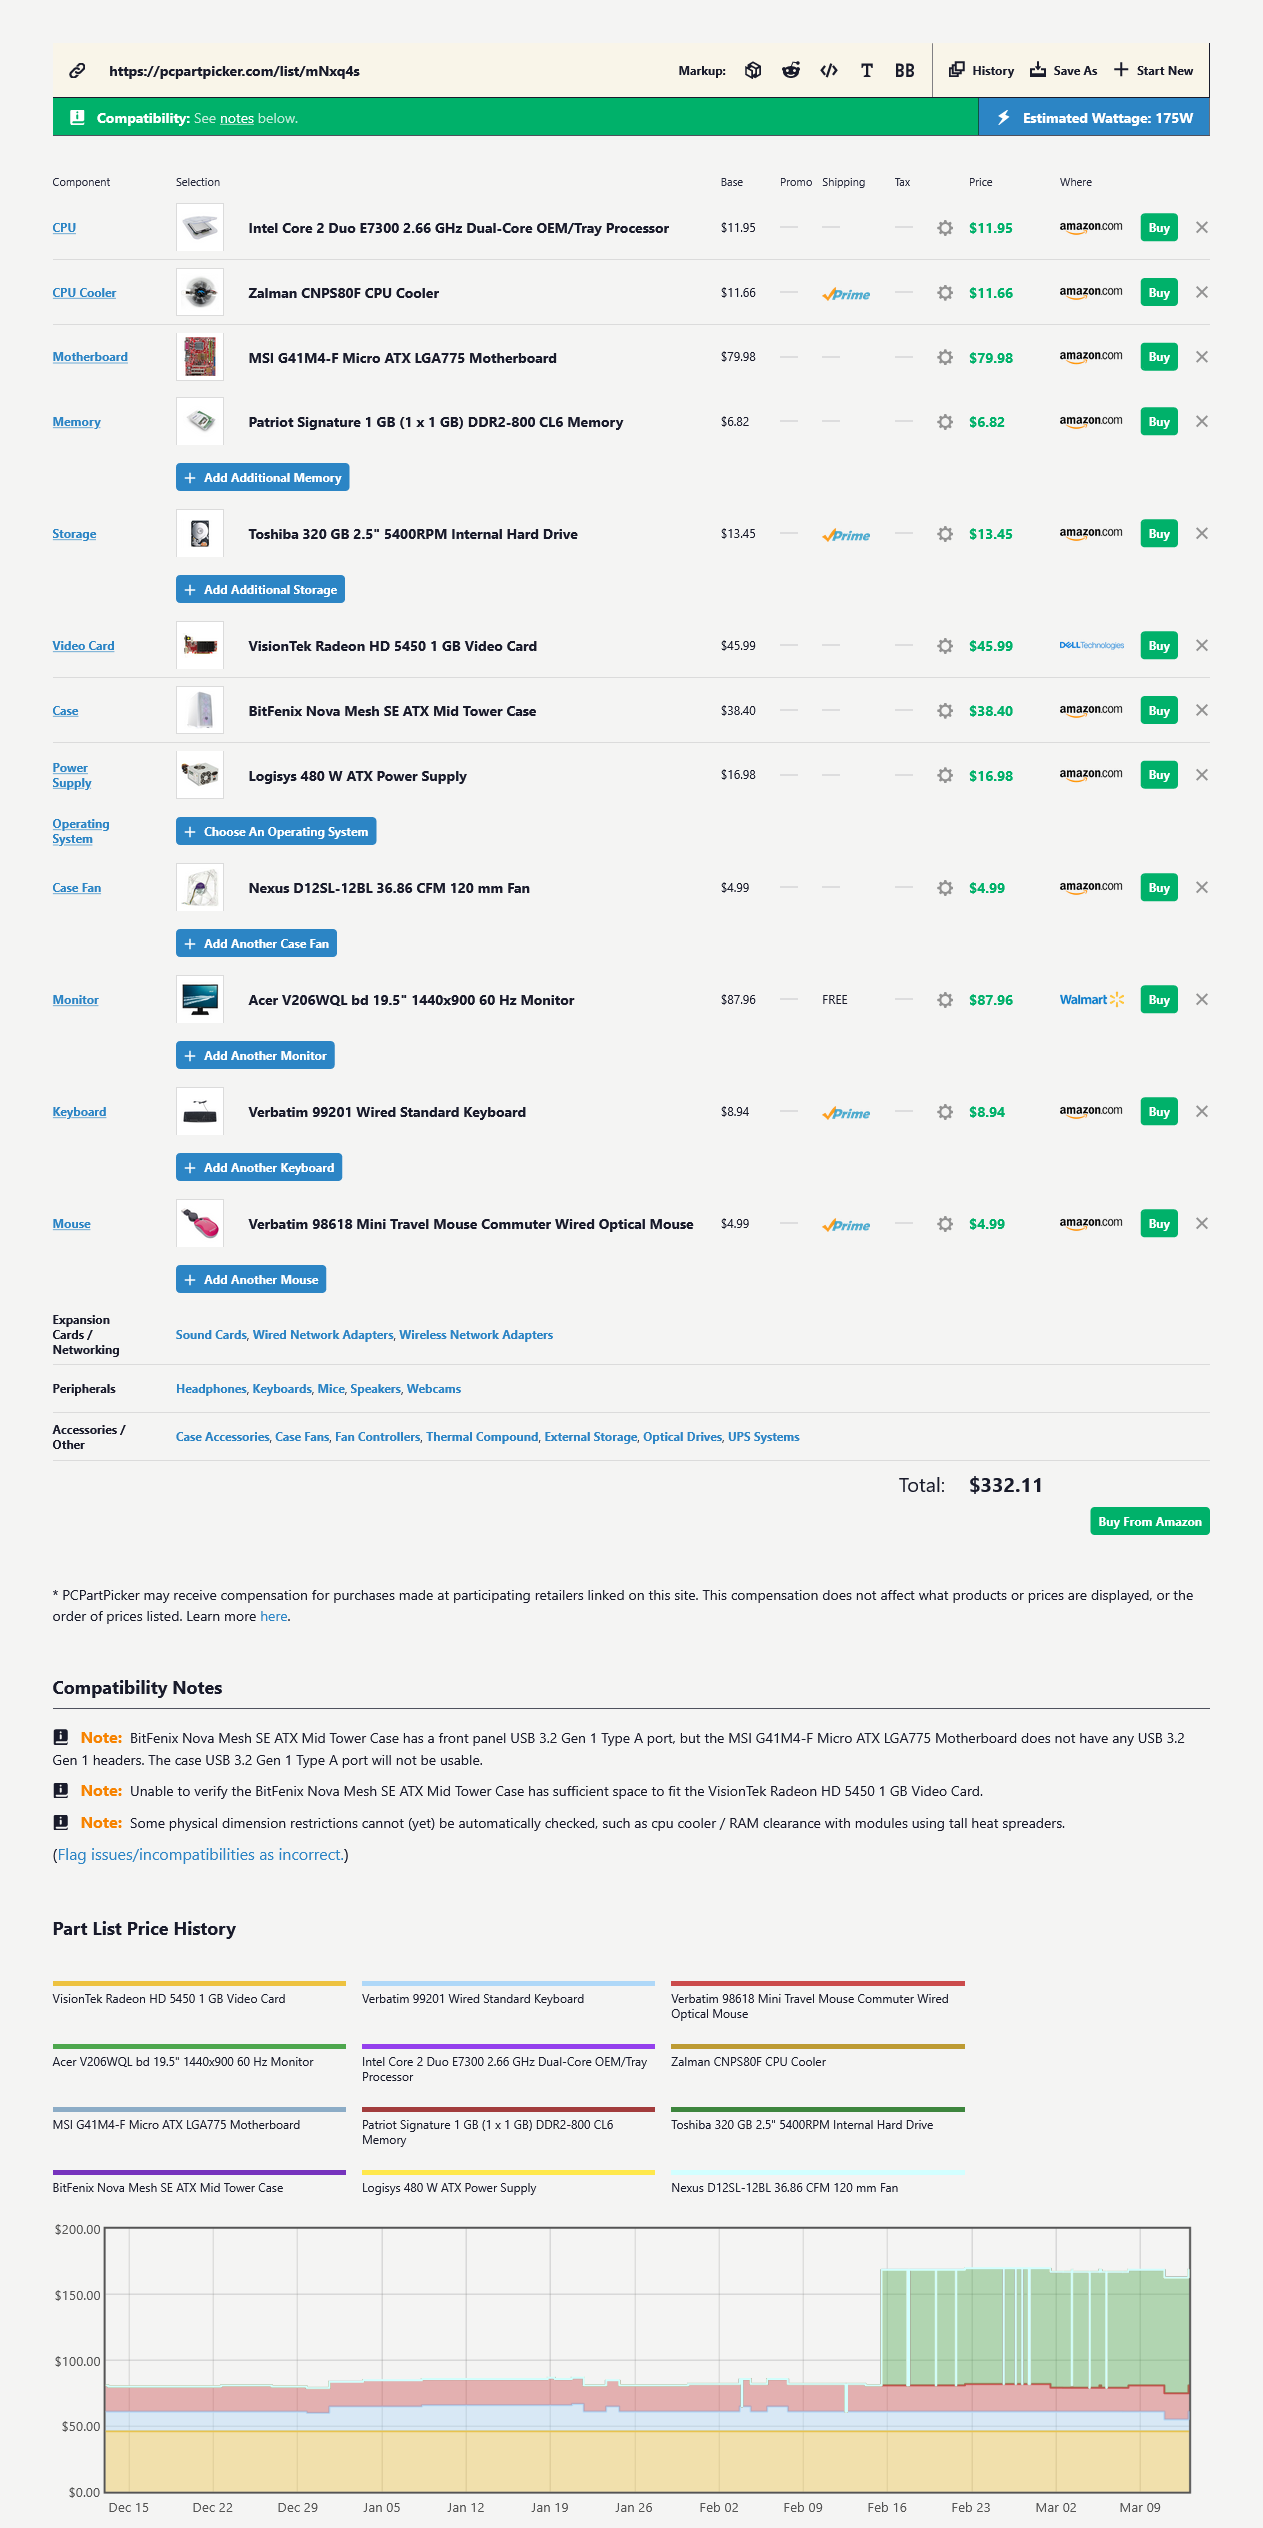
\includegraphics[width=0.6\textwidth]{Minimal.png} \\ \\ \\
La lista de mayor valor: \\
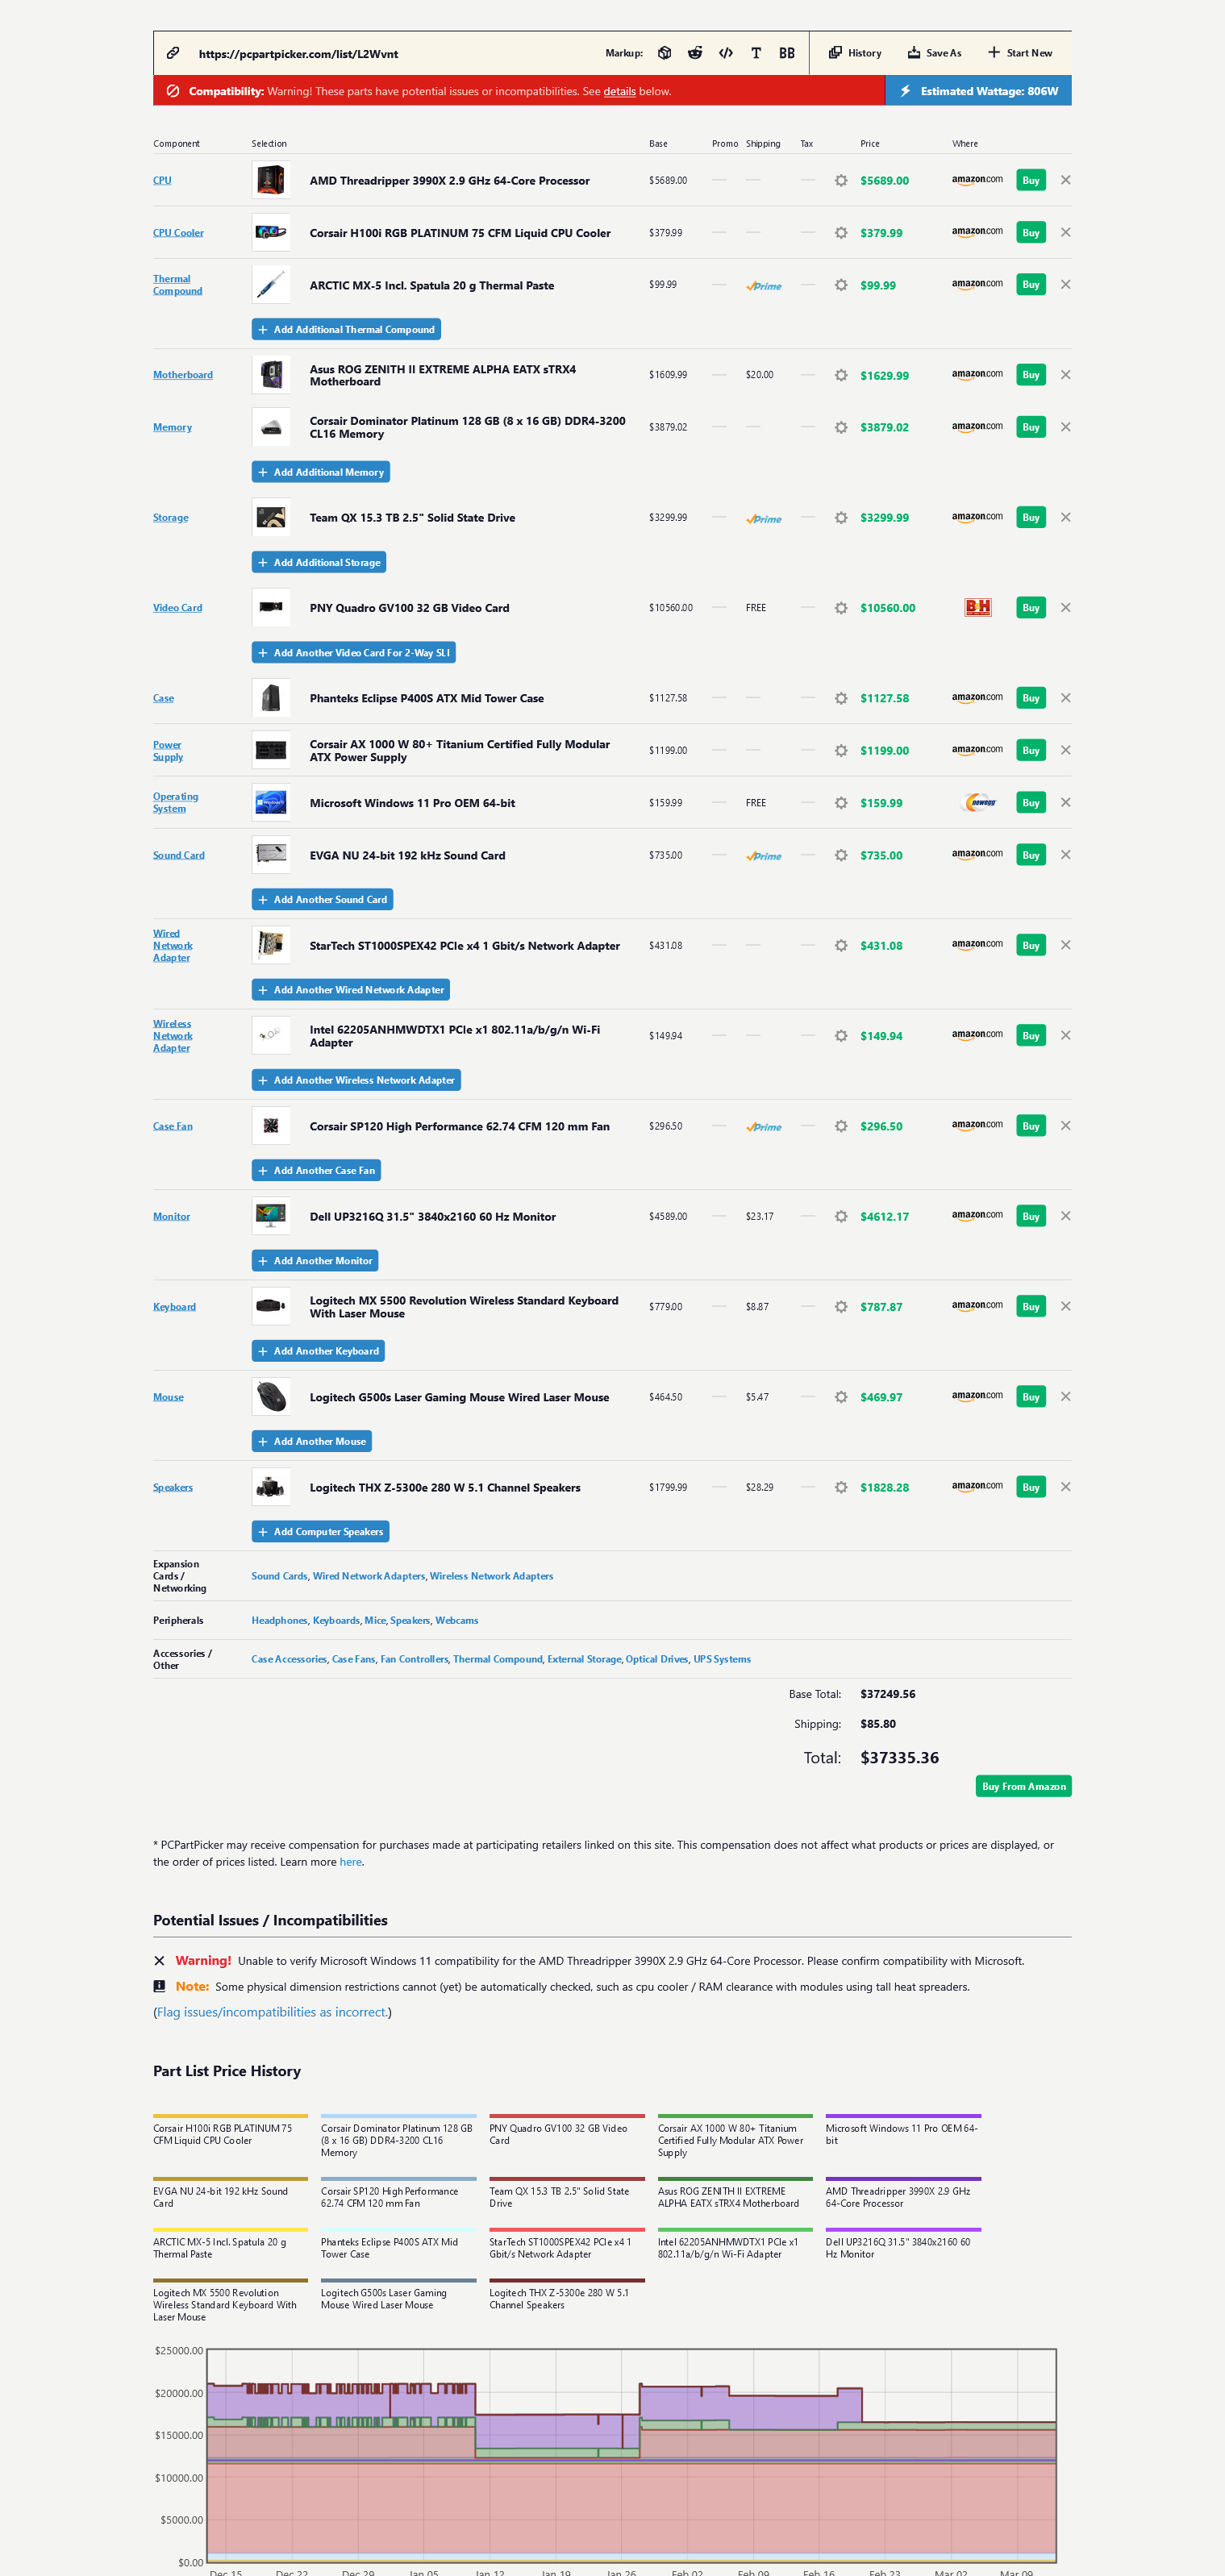
\includegraphics[width=0.6\textwidth]{Maximum.png} \\ \\ \\ \\ \\ \\ \\
La lista ideal de Build Redux: \\
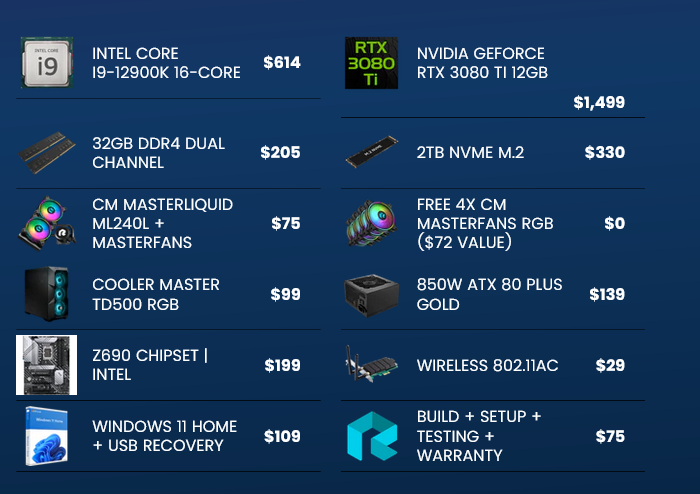
\includegraphics[width=1.2\textwidth]{BuildReduxIdeal.png} \newpage
Las lista ideal de Pc Part Picker: \\ 
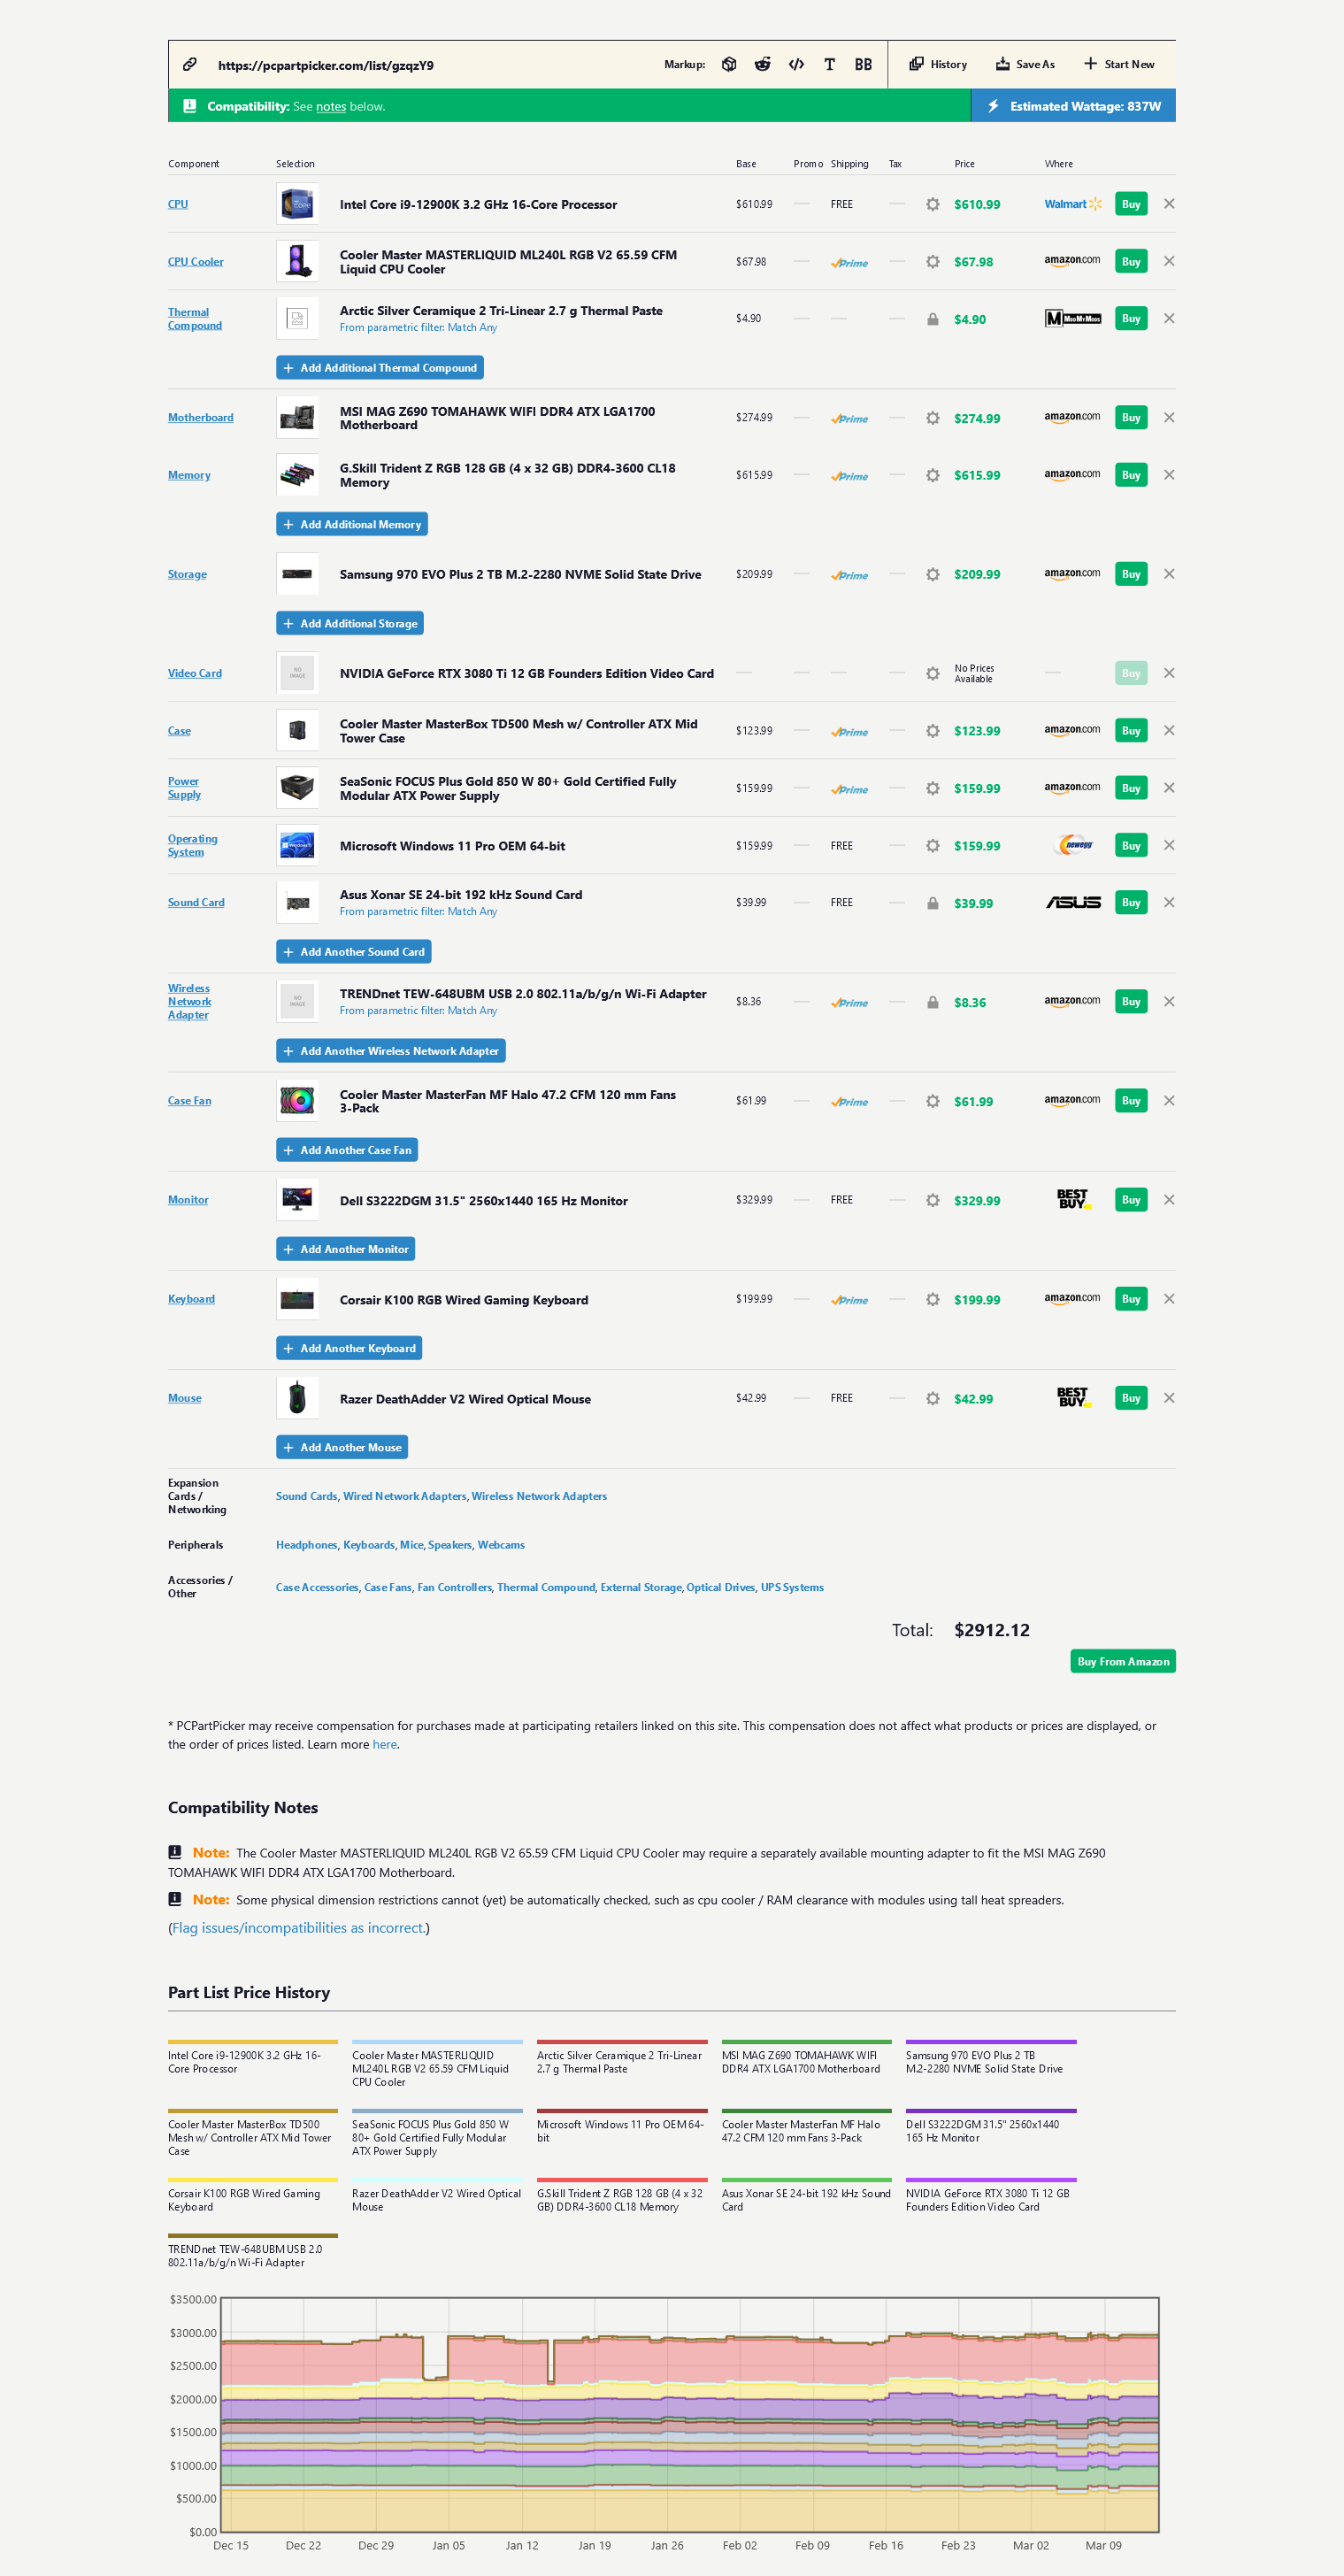
\includegraphics[width=0.6\textwidth]{Ideal.png} \\
\section{Pasos para armar la computadora}
Para esta parte usé un video de referencia para seguir los pasos de como armar una computadora (\cite{linusTechTips_pcbuildingGuide}).
\begin{enumerate}
    \item Asegurese de estar seguro y con antiestática para no dañar los componentes o a si mismo.
    \item Levantar el pestillo, si se puede abrir el zócalo de la CPU (CPU Socket)
    \item Coloque el CPU adentro de zócalo verificando que está en la posición correcta con el indicador del triangulo dorado, si quiere lo intnta agitar para verificar que está colocado bien.
    \item Si puede, cierre el zócalo.
    \item Cierre el pestillo.
    \item Aline la memoria RAM el lugar donde se mete y apriete para abajo hasta escuchar el click, repita con todos los RAM disponibles o hasta acabar espacios de RAM.
    \item Quite el panel del lado del \textit{"Case"} y quite los accesorios, si la tarjeta madre no tiene escudo de I/O isntalelo porque no lo va a poder hacer después.
    \item Coloque la tarjeta madre y asegure que los 9 huecos estan alineados, si no tiene el del centro, puede ser que esta atras, pero cubierto por la armadura (armored plating).
    \item Conecte los cables de poder.
    \item Conecte el audio.
    \item Si tiene avanicos conecte el cable de avanicos.
    \item Conecte el conector de USB 3.0.
    \item Si tiene conector de USB 3.1 gen 2, conectelo.
    \item Si tiene un contector de RBG conectelo.
    \item Que el \textit{"heatsink"} si tiene y si no tiene montadura preinstalada, instalela.
    \item Conecte el SSD en los espacios habilitados en la CPU, si no hay en los lugares del chipset.
    \item Verifique si el \textit{"cooler"} necesita una montadura extra
    \item Ponga los avaincos del frente.
    \item Si necesita agregue la montadura, soquelo con el destornillador y después monte el \textit{"cooler"}, de la CPU.
    \item Quite la tabla que tapa el \textit{"Power Supply"}, conecte los cables de poder que conectó a la tarjeta madre anteriormente, un SATA y si tiene RGB y el \textit{"Power Supply"} que compró le permite conectelo donde debe.
    \item Si la tarjeta gráfica necesita montadura específica agreguela, ingrese firmemente hasta que se conecte a la parte de atras, ajuste con el destornillador.
    \item Si tiene luces para tener por dentro de la PC, conectelos de la tarjeta madra al \textit{"Power Supply"} y conecte los adaptadores y todo al controlador.
    \item Intente de hacer que no se vea desordenado los cables y junte cables con \textit{"zip ties"} y \textit{"cabel ties"}, si quiere los puede nombrar para no confundirse si tiene que entrar a cambiar o modificar después.
    \item Agregue el panel del lado devuelta.
\end{enumerate}

\section{Sistema Operativo}
Como sistema operativo le instalaria Windows 11 con WSL, esto es por la falta de compatibilidad con los juegos en linux, pero WSL me deja programar en Linux que es mejor.
\section{Drivers y Porgramas}
Para los drivers y verificar lo que se necesita busque en este artículo PC Game Heaven (\cite{NecessaryDrivers})
\begin{itemize}
    \item Drivers gráficos, como la tarjeta gráfica es de NVidia instalaría los de NVidia.
    \item Los drivers de la terjeta madre, en este caso es MSI entonces instalaría los drivers que recomienda MSI para la tarjeta madre.
    \item instalaría los drivers para que me sirva el teclado y el mouse bien, drivers de razer y corsair específicamente.
    \item Speedfan y MSI Afterburn, para en ocaciones especiales dejar que sobrecaliente un poco para que no frene el CPU (overclocking)
    \item Hacerle el update a todo lo que necesite, Sistema operativo, drivers, etc.
    \item De momento instalaría VSCode como mi editor de texto para programar, Virtual Code o CLion como IDE, y Steam y Epic Games para instalar juegos, más Discord y Teams para comunicación.
\end{itemize}

\newpage
\printbibliography
\end{document}